\chapter{Logon Logik}
\section{Logon-Szenarien}
Der Logon f�r das System des Sinnesraumes kann �ber zwei Arten erfolgen. Die erste Art ist,
 da� ein Tag durch das OPS innerhalb des Raumes erkannt wurde. Hierf�r meldet das OPS dem Controller alle Tags die den Raum betreten und wieder verlassen. Die zweite M�glichkeit ist der manuelle Logon �ber ein PDA (Eingabe von Benutzernamen und Passwort).
\\
Da immer nur ein Benutzer eingeloggt sein kann, wurde folgendes Rechtekonzept entwickelt, 
um die Logonvarianten zu regeln.

\begin{figure}[!h]
\begin{center}
  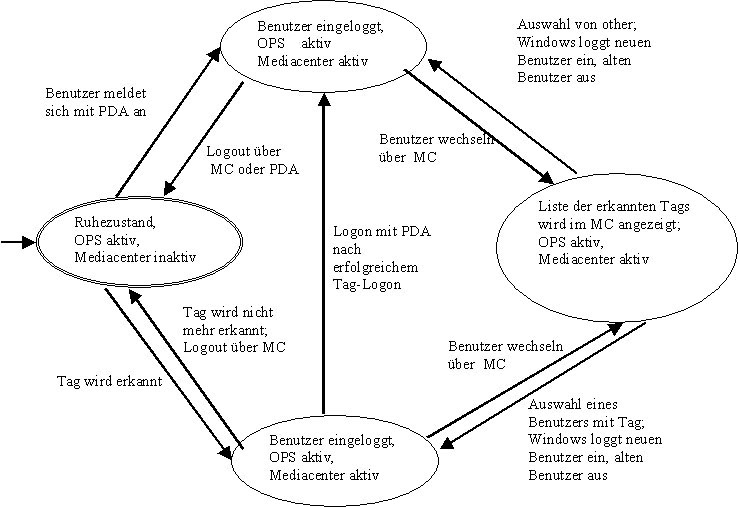
\includegraphics[width=360pt]{positioning.jpg}
  \caption{�bersicht Logon-Szenarien}
\end{center}
\vspace*{-6mm}
\end{figure}

\subsection{Logon aus dem Ruhezustand des Systems (Tagbasiert)}
\subsubsection*{Ausgangssituation}
\begin{itemize}
\item System: Ruhezustand
\item OPS: aktiv
\item Mediacenter: inaktiv
\end{itemize}
\subsubsection*{Logonvorgang}
Der Benutzer, dessen Tag-Id zuerst an den Controller geschickt wird,
wird vom System eingeloggt. Hierzu wird �ber den Controller an das Betriebssystem eine
Nachricht geschickt.
\subsubsection*{Erreichte Situation}
\begin{itemize}
\item System: User eingeloggt (tagbasiert)
\item OPS: aktiv
\item Mediacenter: aktiv
\end{itemize}


\subsection{Logon aus dem Ruhezustand des Systems (PDA-basiert)}
\subsubsection*{Ausgangssituation}
\begin{itemize}
\item System: Ruhezustand
\item OPS: aktiv
\item Mediacenter: inaktiv
\end{itemize}
\subsubsection*{Logonvorgang}
Der Benutzer baut eine Verbindung zwischen seinem PDA und dem Rechner im Sinnesraum auf.\\
Auf der Weboberfl�che seines PDAs kann der Benutzer seinen User-Namen und sein Passwort eingeben.
Dieser wird mit den Daten in der Datenbank �berpr�ft und bei �bereinstimmung der Daten wird der Benutzer 
vom System eingeloggt. Hierzu wird �ber den Controller an das Betriebssystem eine
Nachricht geschickt.\\
Dieser Logonvorgang wird beispielsweise ben�tigt, sollte ein Benutzer sein Tag nicht dabei haben.
\subsubsection*{Erreichte Situation}
\begin{itemize}
\item System: User eingeloggt (PDA-basiert)
\item OPS: aktiv
\item Mediacenter: aktiv
\end{itemize}

\subsection{Change User (Tag-eingeloggt) zu einem anderen Benutzer mit Tag}
\subsubsection*{Ausgangssituation}
\begin{itemize}
\item System: User eingeloggt (tagbasiert)
\item OPS: aktiv 
\item Mediacenter: aktiv
\end{itemize}
\subsubsection*{Logonvorgang}
Der Benutzer hat die M�glichkeit sich �ber das Mediacenter alle Tags, die sich im Raum befinden,  
anzeigen zu lassen. Durch Anklicken des jeweiligen Benutzernamens wird der alte User aus- und der 
ausgew�hlte User eingeloggt.
\subsubsection*{Erreichte Situation}
\begin{itemize}
\item System: User eingeloggt (tagbasiert)
\item OPS: aktiv
\item Mediacenter: aktiv
\end{itemize}

\subsection{Change User (PDA-eingeloggt) zu einem anderen Benutzer mit Tag}
\subsubsection*{Ausgangssituation}
\begin{itemize}
\item System: User eingeloggt (tagbasiert)
\item OPS: aktiv 
\item Mediacenter: aktiv
\end{itemize}
\subsubsection*{Logonvorgang}
Der Benutzer hat die M�glichkeit sich �ber das Mediacenter alle Tags, die sich im Raum befinden,  
anzeigen zu lassen. Durch Anklicken des jeweiligen Benutzernamens wird der alte User aus- und der ausgew�hlte User eingeloggt.
\subsubsection*{Erreichte Situation}
\begin{itemize}
\item System: User eingeloggt (tagbasiert)
\item OPS: aktiv
\item Mediacenter: aktiv
\end{itemize}

\subsection{Change User (Tag-eingeloggt) zu einem anderen Benutzer mit PDA}
\subsubsection*{Ausgangssituation}
\begin{itemize}
\item System: User eingeloggt (tagbasiert)
\item OPS: aktiv 
\item Mediacenter: aktiv
\end{itemize}
\subsubsection*{Logonvorgang}
Der Benutzer hat die M�glichkeit sich �ber das Mediacenter alle Tags, die sich im Raum befinden,  
anzeigen zu lassen. Durch Anklicken von other kann sich mit dem PDA einloggen.
\subsubsection*{Erreichte Situation}
\begin{itemize}
\item System: User eingeloggt (PDA-basiert)
\item OPS: aktiv
\item Mediacenter: aktiv
\end{itemize}

\subsection{Change User (PDA-eingeloggt) zu einem anderen Benutzer mit PDA}
\subsubsection*{Ausgangssituation}
\begin{itemize}
\item System: User eingeloggt (tagbasiert)
\item OPS: aktiv 
\item Mediacenter: aktiv
\end{itemize}
\subsubsection*{Logonvorgang}
Der Benutzer hat die M�glichkeit sich �ber das Mediacenter alle Tags, die sich im Raum befinden,  
anzeigen zu lassen.Durch Anklicken von other kann sich mit dem PDA einloggen. 
\subsubsection*{Erreichte Situation}
\begin{itemize}
\item System: User eingeloggt (PDA-basiert)
\item OPS: aktiv
\item Mediacenter: aktiv
\end{itemize}

\subsection{Logon mit PDA nach erfolgreichem Tag-Logon}
Will ein Benutzer nicht mit dem Trackball navigieren, sondern mit seinem PDA, so kann er sich einfach mit dem PDA einloggen.
\subsubsection*{Ausgangssituation}
\begin{itemize}
\item System: User eingeloggt (tagbasiert)
\item OPS: aktiv 
\item Mediacenter: aktiv
\end{itemize}
\subsubsection*{Logonvorgang}
Der Benutzer verbindet sich mit seinem PDA zum Rechner und gibt sein Benutzernamen
 und sein Passwort ein. Die Daten werden mit denen des eingeloggten Users verglichen.
 Sollte es der identische User sein, so wird er PDA-basiert eingeloggt. Das laufende 
 Programm wird nicht unterbrochen. Sollte es sich um einen anderen User handeln, passiert nichts.
\subsubsection*{Erreichte Situation}
\begin{itemize}
\item System: User eingeloggt (PDA-basiert)
\item OPS: aktiv
\item Mediacenter: aktiv
\end{itemize}

\section{Logoutszenarien}
\subsection{Automatisches Logout eines tagbasierten Users}
\subsubsection*{Ausgangssituation}
\begin{itemize}
\item System: User eingeloggt (tagbasiert)
\item OPS: aktiv 
\item Mediacenter: aktiv
\end{itemize}
\subsubsection*{Logoutvorgang}
Wird das Signal eines tagbasierten Users nicht mehr erkannt, 
so wird dieser automatisch ausgeloggt.
\subsubsection*{Erreichte Situation}
\begin{itemize}
\item System: Ruhezustand
\item OPS: aktiv
\item Mediacenter: inaktiv
\end{itemize}

\subsection{Manuelles Logout eines tagbasierten Users}
\subsubsection*{Ausgangssituation}
\begin{itemize}
\item System: User eingeloggt (tagbasiert)
\item OPS: aktiv 
\item Mediacenter: aktiv
\end{itemize}
\subsubsection*{Logonvorgang}
Ein User kann �ber logout im MediaCenter jeden anderen Benutzer ausloggen. \\
Der User der zuletzt eingeloggt war, kann f�r 30 Sekunden nicht �ber seinen Tag eingeloggt werden.
\subsubsection*{Erreichte Situation}
\begin{itemize}
\item System: Ruhezustand
\item OPS: aktiv
\item Mediacenter: inaktiv
\end{itemize}

\subsection{Logout eines PDA-basierten Users}
\subsubsection*{Ausgangssituation}
\begin{itemize}
\item System: User eingeloggt (PDA-basiert)
\item OPS: inaktiv 
\item Mediacenter: aktiv
\end{itemize}
\subsubsection*{Logonvorgang}
Ein User kann �ber logout im MediaCenter jeden anderen Benutzer ausloggen. Der User kann sich aber auch selbst �ber sein PDA ausloggen.\\
Der User der zuletzt eingeloggt war, kann f�r 30 Sekunden nicht �ber seinen Tag eingeloggt werden.
\subsubsection*{Erreichte Situation}
\begin{itemize}
\item System: Ruhezustand
\item OPS: aktiv
\item Mediacenter: inaktiv
\end{itemize}
